\documentclass[12pt,letterpaper,titlepage]{article}
\usepackage{solarized-light}
\usepackage{fontspec}
\defaultfontfeatures{Mapping=tex-text}
\usepackage{xunicode}
\usepackage{xltxtra}
\usepackage{amsmath}
\usepackage{pdfpages}
\usepackage{amsfonts}
\usepackage{amssymb}
\setcounter{secnumdepth}{0}
\usepackage{nameref}
\usepackage{enumitem}
\usepackage{environ}
\usepackage[pdf]{graphviz}
\usepackage{pdfpages}
\usepackage{pgfplots}
\usepackage{karnaugh-map}

\setmainfont{Times New Roman}
\showboxdepth=\maxdimen
\showboxbreadth=\maxdimen


\usepackage{paracol}
\usepackage{wrapfig}
\globalcounter{table}
\globalcounter{figure}
\usepackage{graphicx}
\usepackage[left=1in,right=1in,top=1in,bottom=1in]{geometry}
\graphicspath{{img/}}

\author{Jacob Abel}
\title{	Project 3B
	\\\large ECE3544 CRN:82989
}

\setlength{\parskip}{0.25em}

\begin{document}
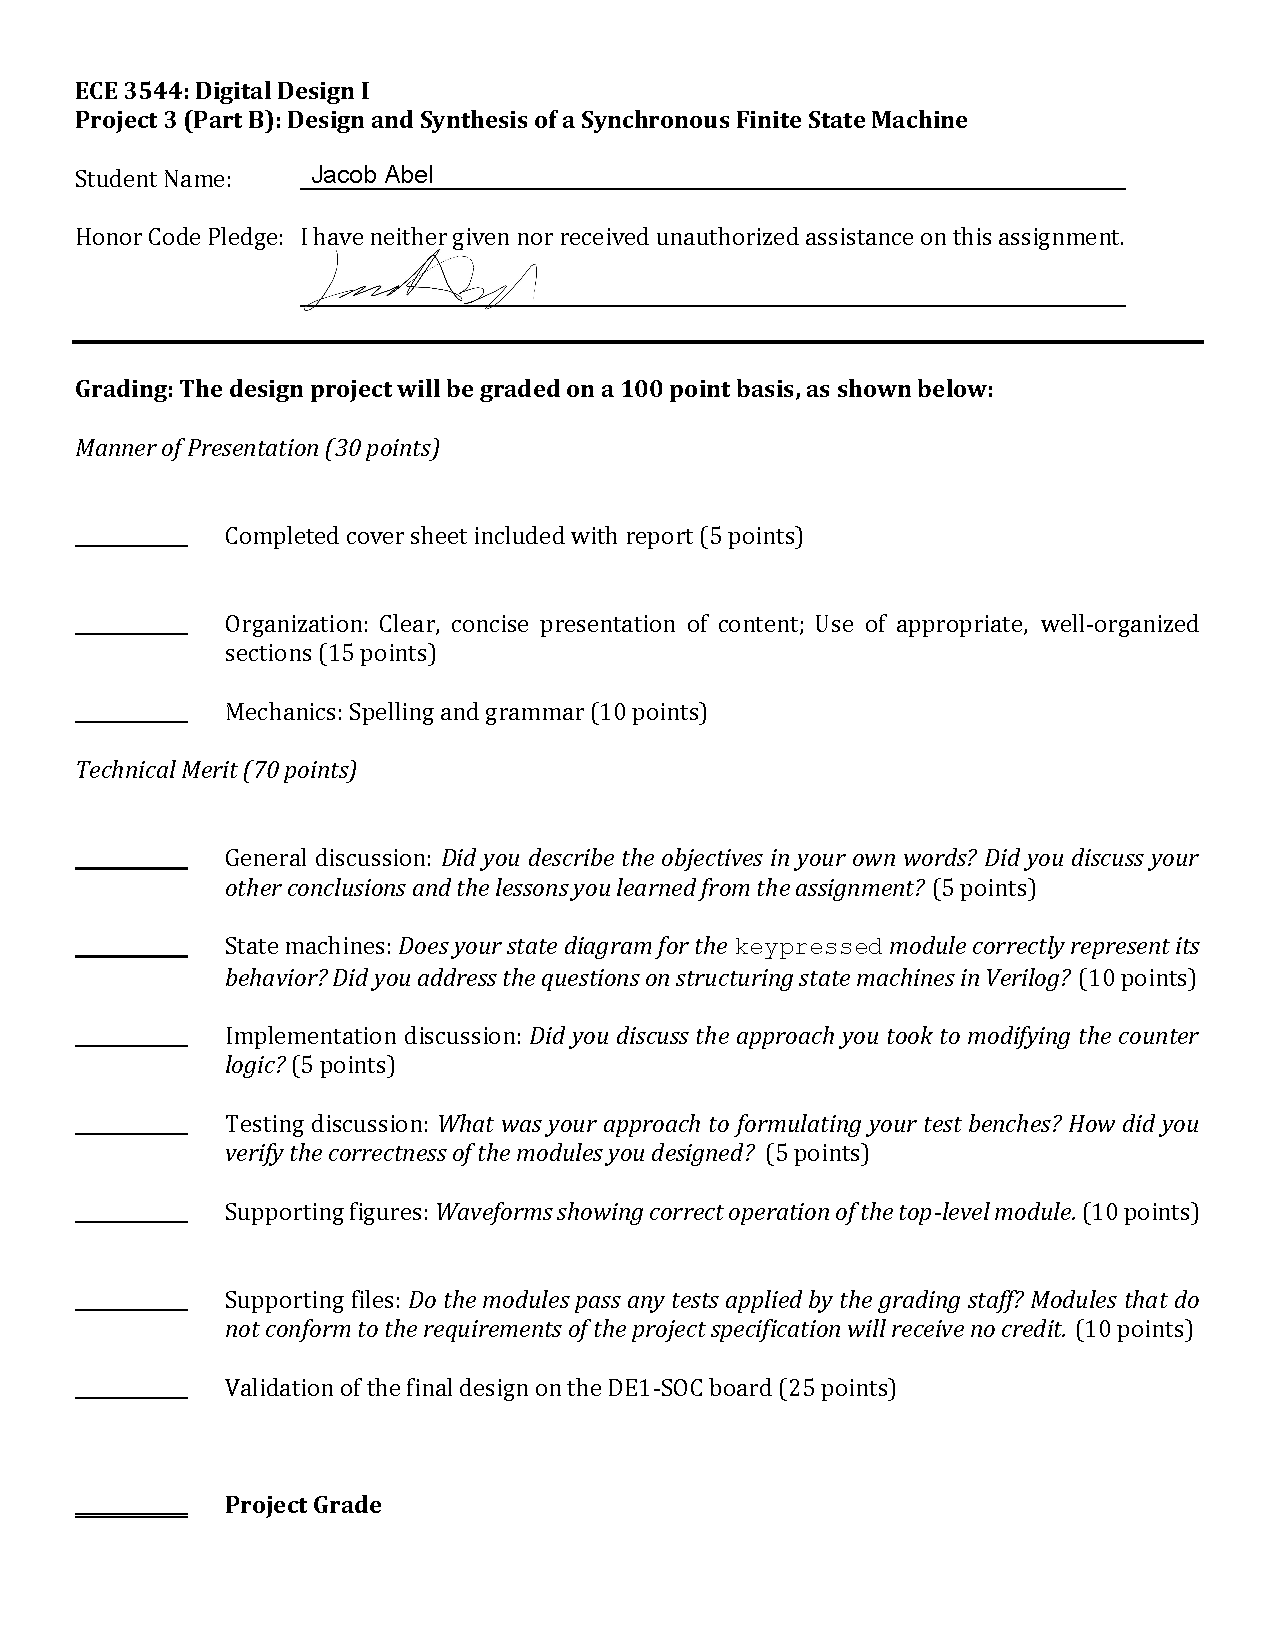
\includepdf[noautoscale]{CoverSheet.pdf}
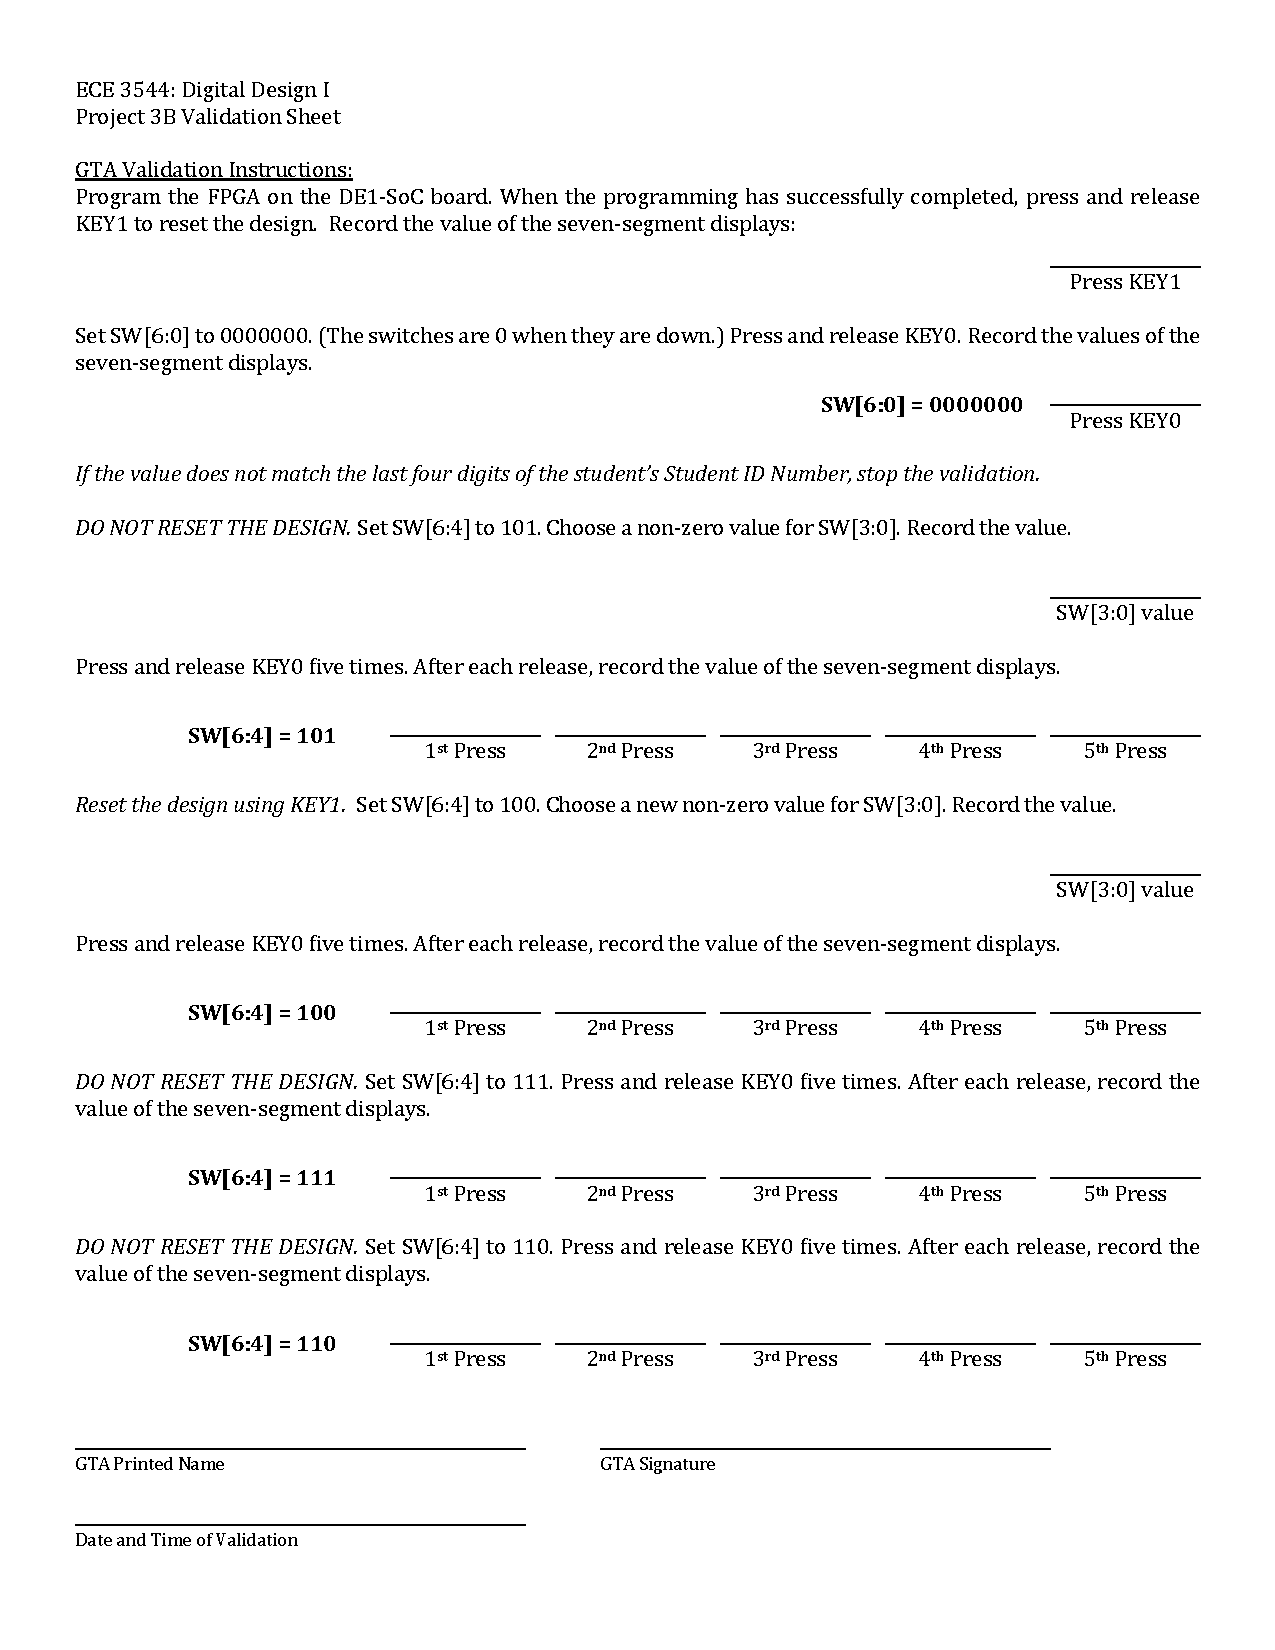
\includepdf[noautoscale]{ValidationSheet.pdf}

\maketitle
\begin{raggedright}

\section*{Objective}
The objective of this project is to demonstrate a capability to synthesise sequential designs onto a real world system such as an FPGA. This project also demonstrates a basic capacity to interpret and implement state diagrams.

\section{Button FSM Diagram}

\begin{figure}[ht]
\centering
\digraph{button}{
	node [shape = plaintext] reset; 
	node [shape = ellipse];
	reset -> KEY_FREE;
	KEY_FREE -> KEY_PRESSED [ label = "    1/0    " ];
	KEY_PRESSED -> KEY_RELEASED [ label = "   1/1    " ];
	KEY_RELEASED -> KEY_FREE [ label = "     X/0" ];
}
\caption{\texttt{keypressed} Module FSM (Input: \texttt{enable\_in}, Output: \texttt{enable\_out})}
\end{figure}

\clearpage
\section{FSM Module Design}
The design process was relatively straightforward. The initial stage is outlining project requirements on scratch paper and verifying it against the official project specification. At this point the starter program was adapted to include 7 segment displays and the proper pin assignments. Functionality of the starter module was verified and the button module was analysed to develop a basic state diagram. Now the final system design started by replacing the bulk of the FSM module with a \texttt{casez} block that corresponded to each stage of the specified state machine. The test-bench was also implemented at this point by walking through the state diagram and matching its output against expected values. Several small bugs were ironed out and the module was tested on the physical device with equivalent functionality.

There were some failed attempts and discoveries made during this project. One attempt was to use the Accellera Open Verification Library which ultimately delayed the project and was removed. Utilising this library will be attempted again with the next project given sufficient time. The discovery was of the usefulness of the \texttt{casez} statement and the restrictiveness of normal \texttt{case} statements. The prior permits wildcard evaluation and is extremely useful.

While the implemented FSM did not follow the standard FSM pattern, due to its simplicity, implementing it as a single procedural always block resulted in significantly cleaner code. A more complex FSM would utilise the standard FSM pattern and be divided into two to three procedural always blocks. The button module opted to use the standard three block pattern with the first block handling internal register states, the second block handling changes of states from inputs, and the final block handling outputs. The primary FSM does all of this in one block with a \texttt{casez} statement.
\clearpage
\section{Project FSM Module Simulation}
\begin{center}
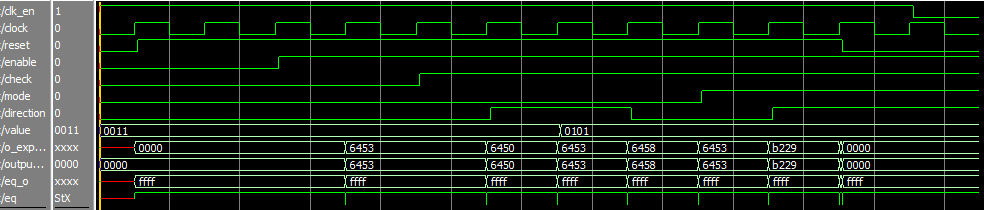
\includegraphics[width=\textwidth]{tb_fsm}

\end{center}

This simulation demonstrates that all the basic inputs produce the correct outputs. The \texttt{reset}, \texttt{enable}, \texttt{check}, \texttt{mode}, \texttt{direction}, and \texttt{value} values are the inputs that compose the switch input values and the \texttt{outputValue} output is the output as 7 segment display values. The \texttt{eq\_} wires demonstrate equivalence on each output pin and the \texttt{eq} wire demonstrates equivalence on all outputs. The equivalences are computed using an XNOR against expected results.

\section{Conclusion}

This project demonstrated the process of implementing, simulating, and physically verifying state machines in Verilog for FPGAs. Despite starting this project early, the project encountered delays due to inexperience during an attempt to utilise the OVL library for the first time. Otherwise, little to no issues arose during the project. As such the project can easily be considered a success with the exception of the the delays due to the lack of experience with the OVL library and the decision to pursue use of said library in lieu of experience.

\end{raggedright}
\end{document}
